\documentclass[utf8, zavrsni]{fer}
\usepackage{booktabs}

% \usepackage{natbib}


% ==== za algo pseudokod
\usepackage{amsmath}
%\usepackage[chapter]{algorithm}
% \usepackage{algorithmic}
\usepackage{minted}
\usemintedstyle{borland}


\usepackage{hyperref}
% \hypersetup{
%     colorlinks,
%     citecolor=black,
%     filecolor=black,
%     linkcolor=black,
%     urlcolor=black
% }
\hypersetup{
    bookmarks=true,         % show bookmarks bar?
    unicode=false,          % non-Latin characters in Acrobat’s bookmarks
    pdftoolbar=true,        % show Acrobat’s toolbar?
    pdfmenubar=true,        % show Acrobat’s menu?
    pdffitwindow=false,     % window fit to page when opened
    pdfstartview={FitH},    % fits the width of the page to the window
    pdftitle={My title},    % title
    pdfauthor={Author},     % author
    pdfsubject={Subject},   % subject of the document
    pdfcreator={Creator},   % creator of the document
    pdfproducer={Producer}, % producer of the document
    pdfkeywords={keyword1, key2, key3}, % list of keywords
    pdfnewwindow=true,      % links in new PDF window
    colorlinks=false,       % false: boxed links; true: colored links
    linkcolor=red,          % color of internal links (change box color with linkbordercolor)
    citecolor=green,        % color of links to bibliography
    filecolor=magenta,      % color of file links
    urlcolor=cyan,           % color of external links
    urlbordercolor={1 1 1}  % color of border around links
}

\graphicspath{{img/}}

\begin{document}

% TODO: Navedite broj rada.
\thesisnumber{000}

% TODO: Navedite naslov rada.
\title{Lanac stranica i distribuirano suglasje u sustavima elektroničkog novca}

% TODO: Navedite vaše ime i prezime.
\author{Bernard Crnković}

\maketitle

% Ispis stranice s napomenom o umetanju izvornika rada. Uklonite naredbu \izvornik ako želite izbaciti tu stranicu.
\izvornik

% Dodavanje zahvale ili prazne stranice. Ako ne želite dodati zahvalu, naredbu ostavite radi prazne stranice.
\zahvala{}

\tableofcontents

% =========================
\chapter{Uvod}
Uslijed procesa globalizacije javlja se sve veća potreba za univerzalnim protokolom novca koji bi zamijenio ili barem objedinio postojeće lokalne bankarske sustave. Zbog loše standardizacije te njene slabe primijene u praksi, javljaju se brojni problemi u poslovanjima banaka što značajno smanjuje propusnost obrade transakcija. Također, mikrotransakcije osjetno su neisplative u sustavima koji imaju visoke naknade za prijenos. Te naknade idejno odgovaraju količini posla za uslugu koju nudi birokratski aparat banke. Cilj je minimizirati i automatizirati količinu posla koja se mora obaviti kako bi mogli vršiti razmjenu novca. Motivirani problemima aktualnih sustava, razmotriti ćemo ideju rješenja trenutnog problema - lanac stranica.

\section{Koncept središnjeg autoriteta}
Pojam \textbf{središnjeg autoriteta} opisuje agenciju ili organizaciju koja osigurava provođenje zakona na međunarodnoj razini\cite{enwiki:969028445}. U ovom nas kontekstu konkretno zanima što taj pojam znači u računarstvu. To je najbolje demonstrirati primjerom koji je u ovoj domeni najčešće asociran s ulogom središnjeg autoriteta: \textbf{Certifikatni autoritet} (engl. \textit{Certificate authority}) - aktor koji se bavi potpisivanje SSL certifikata korištenih u HTTPS protokolu. On ima korijenski samo-potpisani certifikat koji koristi za daljnje potpisivanje zahtjeva (engl. \textit{Certificate Signing Request}). U praksi se obavlja provjeru stvarnog identiteta, odnosno njegovu asocijaciju s certifikatom web poslužitelja drugih firmi koje žele zadobiti povjerenje od klijenata. U samom certifikatu digitalno su potpisane informacije poput javnog ključa korisnika usluge, informacije o tvrtki te vrijeme isteka valjanosti. \textbf{Povezivanjem identiteta fizičke osobe ili organizacije s javnim ključem poslužitelja} osigurava odgovornost (liability) i neporecivost (non-repudiation) u komunikaciji korisnika s vlasnikom certifikata. Ključno je uočiti to svojstvo neporecivosti i povezanosti s identitetom. Samu tajnost komunikacijskog kanala možemo osigurati i bez centralnog tijela (koristeći kriptografske metode za razmjenu ključeva), no ne možemo biti sigurni u identitet druge strane ako prolazimo nesigurnim komunikacijskim kanalom (bez prethodne fizičke interakcije). To je razlog zašto primjerice web preglednici moraju imati unaprijed ugrađene certifikate izdane od vršnih autoriteta (Root CA). Vršni izdavatelji certifikata mogu delegirati to pravo na podređene izdavatelje te tako nastaju \textbf{certifikatni lanci}. Aktualna specifikacija TLS 1.3 mehanizama nalazi se u RFC-8446.


\chapter{Elektronički novac}

Pokazalo se da je u praksi novac najpraktičniji opće prihvaćeni oblik razmjene dobara u obliku trajnog zapisa (u fizičkom ili digitalnom obliku).

\section{Postojeći sustavi novca}
Tradicionalni bankarski sustavi zasnovani su na računalima poslužiteljima koji pohranjuju stanje sustava u relacijskim bazama podataka te upravljaju korisničkim sjednicama, obavljaju autentifikaciju i autorizaciju te barataju transakcijama i stanjima računa. Centralizirana priroda ovakvog sustava osigurava konzistentnost sustava kroz vrijeme, lakše atomične operacije prijenosa sredstava, ali ona ima i neke nedostatke. \\
Naime, pošto ne postoji jedna globalna banka, nastaje problem kako se razmjenjuju sredstva na međunarodnoj razini. Kao primjer jednog rješenja tog problema valjalo bi spomenuti SWIFTNet mrežu \cite{enwiki:1021608159}. SWIFT je osnovan 1973. te je do danas prošao kroz brojne migracije protokola kako bi se od 2001. do 2004. migriralo sa zastarijelog X.25 mrežnog protokola na internet protokol (IP), a kao serijalizacijski format za razmjenu poruka koristi XML. Tada je nastao novi skup standarda (ISO 20022-1: 2004 i ISO 20022-2:2007, Financial services – Universal Financial Industry message scheme). Kasnije je ponovno nadograđivan te je danas on poznat pod nazivom SWIFTNet Phase 2. Taj bi sustav trebao olakšati i u konačnici potpuno standardizirati razmjenu financijskih poruka između banaka u svijetu. Važno je napomenuti da SWIFTNet ne služi za transakcije među bankama već za delegaciju poruka plaćanja lokalnom bankarskom sustavu pri međunarodnoj trgovini. \\ 

Također poznato je da postoje i manje organizacije nalik na SWIFT na razini lokalnih organizacijskih jedinica u državama. Ukratko, većina banaka i dalje ima brojne domenski specifične servise i način funkcioniranja, no ide se prema implementiranju ovog standarda.

\section{Problemi tradicionalnih bankarskih sustava}
	
Može se zaključiti da je financijski sustav iznimno kompleksan, varijabilan. Nestabilan je kroz vrijeme zbog čestih promijena kako bi ostao u koraku s tehnološkim napretkom. Postavlja se pitanje može li se sustav prijenosa financijskih sredstava pojednostaviti, a da zadržimo njegovu pouzdanost (ili ju čak i povećamo). \\

Elektronički sustavi novca zahtijevaju visoku propusnost pri obradi upita, stalnu dostupnost, pouzdanost i otpornost na napade i zlonamjerne vanjske aktore. To su vrlo strogi zahtjevi za bilo koji sustav, a pogotovo za velike sustave koji u poslovnim procesima imaju ljudski faktor (velike birokratski aparat) jer su ljudi skloni pogreškama i kršenju pravila. Osim toga, sama činjenica da je sustav centraliziran znači da postoji točka kvara i svi podređeni čvorovi prestaju funkcionirati što može uzrokovati ogromne štete. Na primjer, ako se sruši kritični bankovni poslužitelj, daljnje transakcije će biti onemogućene za sve korisnike te banke. \\

Druga neželjena nuspojava je potreba za hijerarhijom povjerenja. Naime, čvorovi mreže trebaju vjerovati nadležnima čvorovima te ukoliko je jedan kompromitiran cijelo podstablo takve strukture povjerenja je kompromitirano. Također, kompromis bilo koje financijske institucije u toj strukturi zahtjeva intervenciju pravnog sustava država. \\

Stoga, želimo li koristiti usluge banaka, moramo vjerovati da će ispravno baratati našim financijskim sredstvima.
Unatoč velikoj pouzdanosti, česti su primjeri zakazivanja centraliziranih sustava.

\chapter{Kriptografska podloga}
Prije no što opišemo način funkcioniranja lanca stranica kroz danas najpoznatiju kriptovalutu Bitcoin i demonstriramo postizanje suglasja, važno je definirati korištene kriptografske primitive za njegovu uspješnu implementaciju. Stoga, kada se spominje sažetak ili digitalni potpis, odnosit će se na metode bazirane na sljedećim definicijama.

\section{Funkcija sažetka}
Kriptografska funkcija sažetka $h(x): \{0,1\}^k \rightarrow \{0,1\}^l$ koja ulazu proizvoljne duljine pridružuje determinističku izlaznu vrijednost fiksne duljine. Još se naziva i kompresijska funkcija zato što bilo kakav niz bitova sažima na praktično jedinstven k-bitni identifikator. Željena svojstva te funkcije kako bi se ona smatrala sigurnom su:

\begin{itemize}
	\item ireverzibilnost - poznavajući izlaz $y$ ne možemo odrediti ulaznu vrijednost $m$ tako da vrijedi $y = h(m)$ ako ju prethodno nismo znali
	\item otpornost na kolizije - da svakoj ulaznoj vrijednosti mapira jedinstvenu izlaznu vrijednost, što naravno, nije moguće jer je domena znatno veća od kodomene takve funkcije. Prilikom dizajna teži se što većoj difuziji, tako da su izlazne vrijednosti uniformno raspoređene u prostoru ključeva.
\end{itemize}

\section{Shema digitalnog potpisa}
Digitalni potpis nam služi kako bismo u komunikaciji nesigurnim kanalom mogli osigurati autentičnost poruke našeg sugovornika. To činimo tako da uz svaku poruku koju šaljemo prilažemo jedinstvenu oznaku koja će nakon verifikacije biti dokaz da u tranzitu bitovni informacije nisu bili mijenjani. Formalno, shemu sačinjava trojka $(G, S, V)$ koja predstavlja:
\begin{itemize}
	\item $G(x)$ - funkcija generator para $(k_{s}, k_{v})$ koja kao ulazni parametar prima razinu sigurnosti
	\item $S(m, k_{s})$ - funkcija za potpisivanje koja uz generirani privatni ključ vraća potpis $s$ koji, idealno, jedinstveno odgovara poruci $m$
	\item $V(m, s, k_{v})$ - funkcija verifikacije ispravnosti potpisa koja pomoću $k_{v}$ vraća logičku istinu ili laž ovisno o tome je li $s$ zaista potpis od $m$
\end{itemize}
Kako bismo ju smatrali sigurnom ona mora zadovoljavati pružati sljedeće kvalitete:
\begin{itemize}
	\item Autentifikaciju potpisatelja poruke (osigurava identitet)
	\item Integritet - mogućnost otkrivanja ukoliko je poruka bila mijenjana prilikom slanja (to slijedi direktno iz otpornosti potpisa na kolizije)
	\item Neporecivost - ne može se poreći potpisivanje poruke koja je vezana uz nečij javni ključ. To sljedi i iz nekrivotvorivosti potpisa, odnosno veza između ključa i potpisa je jedinstvena.
\end{itemize}

\chapter{Lanac stranica}
Lanac stranica općeniti je naziv za jednu od metoda implementacije mreže ravnopravnih sudionika bez nadležnog autoriteta za postizanje suglasja. On može imati različite primijene (monetarni sustavi, ugovori, glasovanje, prodaja digitalnih dobara, osiguranje autorskih prava, sigurnu pohranu podataka i brojni drugi...) Povjerenje koje tradicionalno dajemo nekom centralnom tijelu, sada se premješta na povjerenje u kriptografske primitive koje su dokazano pouzdane te ne sadržavaju ljudski faktor sklon pogreškama.

Lanac stranica metoda je koja izjednačuje identitet sa samim kriptografskim ključem i time eliminira potrebu za središnjim autoritetom koji bi regulirao identitet. Suglasje oko globalnog stanja sustava postiže se glasovanjem legitimnih\footnotemark čvorova mreže. (ono što vjeruje većina čvorova mreže, smatra se pravim stanjem).

Stranice u lancu sadrže podatke o stanju mreže te opisuju sve nove događaje u njoj. Temeljem njihovih informacija donose se buduće odluke na lancu. Kaže se da su stranice povezane u lanac zato što su ulančane svojim kriptografskim sažetcima - odnosno, svaki sljedeći lanac sadrži u sebi informaciju sažetka prethodnog lanca. To služi za očuvanje integriteta lanca stranica u slučaju pogrešaka ili namjernih pokušaja napada.

\footnotetext{Legitimnim čvorom smatra se svaki čvor koji je kompatibilan sa specifikacijom sustava, odnosno poštuje sva pravila ispravne komunikacije s drugim čvorovima (to ga i dalje ne sprečava da pokuša zlonamjerno komunicirati s ostalim sudionicima)}

% ==========================
\section{Bitcoin}
\subsection{Ključevi}
Bitcoin mreža koristi ECDSA secp256k1 eliptičnu krivulju kao osnovni algoritam za potpisivanje transakcija u binarnom DER formatu.
\subsection{Adrese}
Adresa $A$ u Bitcoin mreži su efektivno sažetci javnih ključeva. \textit{SHA256} i \textit{RIPE160} predstavljaju kriptografske funkcije sažetka. Verzija protokola je uključena u izračun kako nebi došlo kolizija sa adresama iz drugih kriptovaluta nastalih na Bitcoin mreži kao podlozi. Izračunava se kao
\begin{equation} \label{eq2}
\begin{split}
K_{hash} &= V \mathbin\Vert \mathrm{RIPEMD160}(\mathrm{SHA256}(K_{pub})) \\
C_{sum}  &= \mathrm{SHA256}(\mathrm{SHA256}(K_{hash})) \\
A        &= \mathrm{BASE58}(K_{hash} \mathbin\Vert C_{sum})
\end{split}
\end{equation}
gdje $ V $ označava verziju protokola.

\subsection{Merkleovo stablo}
Struktura podataka nazvana po znanstveniku Ralphu Merkleu koji ju je patentirao 1979. godine. Ona je binarno stablo sažetaka u kojem su listovi obični sažetci blokova podataka a svaki roditelj ima dvoje djece čiji se sažetak računa kao $$ H(H(C_{left}) \mathbin\Vert H(C_{right})) $$.
\subsection{Stranica}
Stranica je struktura podataka koja ima rezervirana specijalna polja za sljedeće informacije:
\begin{itemize}
    \item verziju protokola
    \item \textbf{sažetak prethodne stranice}
    \item sažetak korijena Merkleovog stabla transakcija
    \item oznaku vremena nastanka bloka u UNIX formatu
    \item izračunatu cjelobrojnu vrijednost $ N $ težine mreže
    \item pronađeni slučajni broj koji sadržava $ N $ vodećih nul-bitova
    \item varijabilni cijeli broj $ T $
    \item polje od $ T $ transakcija (najčešće veličine 1-2 MB)
\end{itemize}

\subsection{Transakcija}
Transakcije u Bitcoin mreži organizirane su u takozvane nepotrošene izlaze (engl. \textit{UTXO - Unspent Transaction Output}) koji se sastoje od varijabilnog broja ulaza (\textit{TxIn}) i 2 izlaza (\textit{TxOut})

% =========================

\subsection{Validacija transakcija digitalnim potpisima}
Bitcoin, nesumnjivo vodeća kriptovaluta današnjice, jedan je od jednostavnijih primjera implementacije protokola za digitalni novac temeljen na ideji lanca stranica. Objasnit ćemo ukratko ideju rada Bitcoina i njegova ograničenja. Čvorovi Bitcoin mreže postižu suglasje takozvanim rudarenjem što je zapravo uzastopno ponavljanje operacija izračunavanja SHA-256 sažetka stranice (engl. \textit{ledger}) konkateniranog s nekom vrijednosti koju rudar mora pronaći kako bi zadovoljio zahtjev mreže - a to je da konačni sažetak ima prefiks od $N$ 0-bitova. Broj N zove se težina (difficulty) te je on direktno povezan s vjerojatnošću pronalaženja takvog sažetka. To se radi kako bi čvor koji uspješno pronađe taj sažetak mogao dokazati ostatku mreže da je on (u prosjeku) uložio vrijeme proporcionalno broju zahtjevanih prefiks nula. Ostatak mreže mu mora vjerovati jer ne postoji prečica kojom bi se predvidjela vrijednost funkcije sažetka bez da ju zapravo provedemo. Integritet Bitcoin lanca oslanja se na uvjerenje da je SHA-256 kriptografski sigurna funkcija sažetka. Opisat ćemo u nekoliko koraka proces kojim bi zamišljeni aktori Alice i Bob proveli transakciju u Bitcoin mreži:
\begin{enumerate}
	\item Alice i Bob izgeneriraju kriptografske ključeve shemom digitalnog potpisa.
	\item Alice izradi transakciju u kojoj navodi da šalje Bob-u određeni iznos novaca. Alice zatim potpiše tu izjavu (claim) svojim tajnim ključem te ju objavi u mrežu
	
	\item Čin objave transakcije je zapravo kontaktiranje čvorova u mreži koji se bave rudarenjem te se Alice-ina transakcija dodaje na listu nepotvrđenih transakcija\footnotemark
	\footnotetext{Unconfirmed transaction pool je bazen (prioritetni red nepotvrđenih transakcija koje se trebaju obraditi). On je sortiran tako da rudar iz njega uzima transakcije koje njemu donose najveći profit te ih validira i dodaje na popis u sljedeću stranicu koju treba izrudariti.}
	
	\item Rudar će, iz prioritetnog reda sortiranog po veličini naknade za svoju uslugu\footnotemark uzimati transakcije, provjeriti ispravnost potpisa te njihovu odgovaraju li oni zapisima u bazi povijesti lanca stranica
	\footnotetext{Transaction fee je relativn mali iznos koji plaćamo rudaru za njegovu uslugu potvrđivanja naše transakcije kako bi on imao motivaciju raditi svoj posao}
	
	\item Ako je transakcija ispravna, rudar dodaje transakciju na popis u sljedeću stranicu u lancu koju treba 'izrudariti'
	\item Važeće transakcije spremaju se u binarno stablo gdje je roditeljski sažetak jednak sažetku oba sažetka djece\footnotemark. Takva struktura podataka olakšava izračunavanje SHA sažetka bez da moramo trošiti vrijeme na ponovno izračunavanje svih starih SHA-256 sažetaka prijašnjih transakcija u stablu koje stalno raste. Pri dodavanju novih transakcija moramo samo Ažurirati jednu granu u tom stablu koja vodi do korijenskog sažetka koji u konačnici završava u opisniku stranice zajedno sa zaglavljem stranice, i odredišnom adresom rudara
	\footnotetext{Merkle tree ili u Ethereum mreži Patricia (prefix) trie je}
	
	\item U stranici postoji mjesto rezervirano za poseban broj kojeg rudar traži grubom silom tako da sažetak opisnika stranice ima svojstvo koje zahtjeva mreža (N vodećih nul-bitova)\footnotemark
	\footnotetext{Difficulty ili zahtjevnost mreže je broj vodećih 0-bitova koje sažetak lanca mora sadržavati}
	\item Uslijed pronalaženja sažetka s odgovarajućom zahtjevnošću, on objavljuje svoju stranicu susjednim čvorovima i na taj se način nova stranica propagira kroz mrežu. Svi čvorovi preuzmu novu stranicu, prestaju sa traženjem svojeg broja te ponovno grade novu stranicu na upravo primljenoj stranici.
	\item Čvorovi koji još nisu čuli za novu stranicu, nastavljaju se natjecati s njom. Ukoliko dođe do istovremenog rudarenja više jednakovrijednih stranica na različitim računalima, onaj koji se uspije propagirati na više čvorova ima veće izglede da će izrudariti i sljedeću stranicu zasnovanu na toj stranici te time 'pobijediti'\footnotemark \footnotemark. Prosječno vrijeme potrebno za nastanak nove stranice u Bitcoin mreži je 10 minuta (dok neki lanci stranica poput Ethereuma imaju znatno kraće vrijeme od 14 sekundi). Stoga je privremeno račvanje češća pojava u Ethereum mreži.
	\footnotetext{Orphaned block je stranica koja je odbačena zato jer je započela kraću granu u lancu, a prema suglasju mreže, uvijek moramo graditi na najduljem lancu jer je on autoritativan te prikazuje stvarno stanje mreže. Trasakcije na odbačenim stranicama postaju nevažeće. To je jedan od razloga zašto se savjetuje da se pričeka nekoliko blokova prije nego što se vjeruje posljednjoj izrudarenoj stranici}
	\footnotetext{Forking ili račvanje je trenutak kada se još ne zna pravo stanje mreže zbog dvije stranice nastale u bliskom vremenskom okviru. To se relativno brzo razrješava rudarenjem već sljedeće stranice nakon jedne od njih}
\end{enumerate}

\section{Ispravnost tvrdnji u lancu stranica}
Rudari moraju imati bazu podataka o povijesti lanca stranica te asocirane adrese uz javne ključeve za digitalne potpise transakcija\footnotemark. Također moraju pratiti nepotrošene izlaze transakcija. Sam bitcoin ne specificira implementaciju takvih baza podataka, no teži se korištenju što bolje optimizacije (indeksiranja) lanca kako bi rudari ostali kompetitivni s ostatkom mreže. Također postoje i čvorovi koji nude samo uslugu pretraživanja baze ili ogledala (mirroring). Primjerice, najpopularnija implementacija baze podataka za Bitcoin čvor koristi Google-ov LevelDB bazu podataka koja nudi brzi pristup disku u strukturi asocijativnog polja.
\footnotetext{ Takozvani Full-Node je čvor koji čuva arhivu povijesti cijelog lanca u svrhu validiranja ispravnosti budućih transakcija, čuvanje javnih ključeva drugih korisnika za provjeravanje i izračunavanje }

Transfer valute u Bitcoin mreži provodi se kroz takozvane nepotrošene izlaze transakcija\footnotemark. Svaki nepotrošeni izlaz transakcija je asociran s jednim vlasnikom (kriptografskim javnim ključem) te ga može samo vlasnik odgovarajućeg privatnog ključa poslati na neku drugu adresu. Prilikom toga, nepotrošeni izlaz može biti raspoređen na više odredišta. Stoga ako pošiljatelj ne želi poslati cijeli iznos nepotrošenog izlaza transakcije, mora svoju adresu navesti kao odredište za ostatak iznosa koji nije poslan primatelju.
\footnotetext{Unspent Transaction Output (UTXO) je zapis koji uz sebe ima asocirane ulaze odnosno količine uplaćenog novca s jedne ili više adresa te dva izlaza koji određuju odredišne adrese. Dva izlaza služe kako bi se mogao poslati samo dio sredstava na neku drugu adresu a ostatak usmjeriti natrag u vlastitu. Skup svih nepotrošenih izlaza transakcija je valuta u cirkulaciji.}

\section{Dokaz rada}
Dokaz rada je osmišljen kako bi se onemogućilo zlonamjernim čvorovima da razglasuju pogrešne informacije o stanju mreže (primjer: razglase da imaju više bitcoin-a u svom vlasništvu ili više puta potroše iste bitcoin-e koje posjeduju). Dokaz rada fizički onemogućava takve pokušaje varanja zato što bi za takvo što napadač morao imati većinu računalne snage u mreži što svakako nije moguće. Međutim centralizacija je i dalje velik problem u ovakvim mrežama jer kompanije s najjačom opremom imaju najveće izglede za pronači sažetak sljedećeg bloka. Poticaj rudarima na obavljaju taj zahtjevan posao je činjenica da će prema dogovoru specifikacije biti nagrađeni određenim iznosom kriptovalute\footnotemark
\footnotetext{Block reward}
Kako bi rudari imali interesa uopće uključivati transakcije i graditi Merkle stabla, biti će dodatno nagrađeni i od svake obrađene transakcije prema informaciji koju je izdavatelj odredio. Zato su transakcije organizirane u prioritetni red - rudarima se više isplati prvo obrađivati transakcije sa višom naknadom te će one prije biti potvrđene. Moguć je scenarij da transakcije nikada ne budu uključene na popis stranice jer imaju prenisku naknadu, a u red prevelikom brzinom dolaze nove transakcije. Međutim, ne možemo biti sigurni da nikada neće biti potvrđena transakcija sa niskom naknadom. Mehanizam otkazivanja transakcija ne postoji te je velik rizik ostaviti ju u bazenu. Novac se može \textit{spasiti} dvostrukom potrošnjom\footnotemark na drugi vlastiti račun uz znatno višu naknadu kako bi bila potvrđena prije navedene 'spore' transakcije.
\footnotetext{Double spending}

\subsection{Negativne strane dokaza rada}
U teoretskom napadu\footnotemark od 51\% snage radi se upravo o tome da grupa koordiniranih zlonamjernih čvorova može zamrznuti ostale rudare od natjecanja za sljedeću stranicu. Kada bi se našla takva hipotetska organizacija, ništa ju ne bi moglo zaustaviti i ne postoji pravi način da se mreža zaštiti od takvog napada. Oni bi mogli generirati prazne stranice (što je potpuno legalno) te ih periodički propuštati ostatku mreže kako bi odustali od svojeg uzaludnog rada. Sav rad poštenih čvorova u mreži bio bi uzaludan i stranice bi bile važeće i prazne. Ovaj se napad najčešće zanemaruje zbog neizglednosti da će jedna organizacija ikad imati procesorsku većinu. Međutim, statistike pokazuju drugačije - distribucija računalne snage između koordiniranih rudarskih bazena je vrlo segregirana i postoji stvarna prijetnja od ovakvog napada. Mreža nije toliko decentralizirana koliko je bilo planirano.
\footnotetext{51\% Attack...}

\subsection{O vremenu stranice u Bitcoin mreži}
Bitcoin ima samo-podesivi mehanizam ugrađen u protokol koji brine da je prosječno vrijeme za pronalaženje sažetka sljedeće stranice bude oko 10 minuta. Međutim, novi čvorovi nastaju u mreži, a neki postojeći se gase te stoga ukupna komputacijska snaga doživljava stalne fluktuacije. Rješenje za taj problem je da se broj zahtjevanih vodećih nul-bitova u bloku prilagođava obrnuto proporcionalno prosječnom vremenu mreže svakih 2016 stranica (što je okvirno 2 tjedna). Svaki rudar taj broj može nezavisno izračunati te prilagoditi svoj ciljani broj vodećih nul-bitova koje traži. Na taj način je osigurano približno konstantno vrijeme stranice. 

\section{Dokaz uloga}
Zbog neekonomičnosti mehanizma dokaza rada, koji izaziva veliko opterećenje računalnih sustava a posljedično i troši veliku količinu električne energije, javile su se nove metode postizanja suglasja u mrežama bez dokaza rada. Dokaz uloga\footnotemark \footnotetext{Proof of Stake...}
je možda najpoznatija alternativa.Idejno on radi tako da se čvorovi validatori u mreži kandidiraju te uz vjerojatnost proporcionalnu njihovom ulogu u pametnom ugovoru, bivaju izabrani da validiraju sljedeću stranicu i time dobivaju nagradu. Pri pokušajima varanja, napadač bi trebao biti kažnjen prema suglasju mreže tako da mu se velik dio njegovog uloga oduzme što napade čini vrlo nepraktičnima. Cardano (ADA)\footnotemark \footnotetext{} je kriptovaluta koja se od svog početka oslanja na ovakav način rada, a Ethereum, unatoč tome što se oslanja na  (ETH) ima eksponencijalno povećanje složenosti svakih 100.000 stranica kako bi potaknuo što bržu tranziciju mreže na dokaz uloga. \cite{wood2014ethereum}.

% Premijestil sam ovo tu jer objašnjavam od jednostavnihih koncepti prema složenijima.
\section{Metode postizanja suglasja u sustavima bez povjerenja}
Čvorovi mreže moraju biti u suglasju oko stanja sustava kako bi mogli donositi odluke o svojim budućim akcijama. Dakle, moraju svi dijeliti isti lanac stranica. To se postiže odbacivanjem svih drugih lanaca osim autoritativnog. Odluka o tome koji je lanac autoritativan donosi se na temelju većine računalne moći iz čega sljedi i najdulji lanac. Ako u bilo kojem trenutku nastanu dvije nove stranice te se propagiraju mrežom (to se naziva račvanje lanca \textit{forking}), jedna od njih će imati većinu rudarske snage. Prije no što se ispostavi koja je ispravna, one su jednakovrijedne i upravo zbog toga se ne vjeruje posljednjoj stranici u lancu. Vjerojatnost za takvu neizvjesnost u lancu je vrlo niska te opada eksponencijalnom brzinom ukoliko napadač posjeduje manjinu snage u mreži \cite{btc, satoshi}.
\begin{itemize}
	\item Lanac stranica je robustan u smislu da je otporan na greške u sustavima zbog decentraliziranosti (Mreža radi čak i kad bilo koji pravi podskup čvorova zakaže).
\end{itemize}

% =========================
\chapter{Simulacija postizanja suglasja}

U ovom ćemo poglavlju izraditi demonstracijski softver kako bismo simulirali postizanje konsenzusa u lancu stranica u mreži s više sudionika. Koristit ćemo metodu koju koristi i Bitcoin mreža jer 

\section{Opis}
Implementacija je ostvarena u programskim jezicima Python i Javascript. Sastoji se od dva dijela. Backend-a čvora koji je zapravo poslužitelj s kojim komuniciramo HTTP protokolom preko REST metoda. Poslužitelj je napisan u radnom okviru Flask. Za ostvarenje spremišta ključeva, korištene su kriptografske primitive iz knjižnice PyCryptodome. Drugi dio implementacije sastoji se od front-end klijenta kojemu pristupamo kroz web preglednik. Naravno, korišten je programski jezik Javascript bez dodatnih knjižnica. Korišten je standardni asinkroni API zasnovan na obećanjima i fetch upitima koji će pozivati Flask back-end našeg čvora. Zajedno ta dva dijela čine jedan čvor u mreži. Možemo instalirati softver na više računala te simulirati njihovu međusobnu interakcij: postizanje suglasja i vršenje transakcija. Serijalizacijski format korišten za komunikaciju je JSON.

\section{Izrada transakcija}

\subsection{Adrese}
Adrese digitalnih novčanika u ovoj se simulaciji izračunavaju kao SHA-256 sažetak javnog ključa čvora nakon njihove serijalizacije u PEM (ascii) kodiranu DER strukturu javnog ključa. Adresa kao sažetak javnog ključa uobičajena je praksa u popularnim implementacijama lanca stranica.

\subsection{Struktura transakcije}
Transakciju na vrlo jednostavan način stvaramo u web pregledniku tako da unesemo odredišnu adresu i iznos koji želimo poslati na tu adresu. Tijelo upita u implementaciji formatirano je na sljedeći način:
\begin{minted}[obeytabs=true,tabsize=4,frame=single,framesep=10pt]{json}
{
	"data": {
		"amount": 35,
		"block_index": 5,
		"dst": "<heksadekadska_adresa_pošiljatelja>",
		"src": "<heksadekadska_adresa_primatelja>"
	},
	"pub_key": "-----BEGIN PUBLIC KEY-----...",
	"signature": "<heksadekadski_potpis_pošiljatelja>"
}
\end{minted}

Slanje čvoru (poslužitelju/rudaru) upit za stavljanje nove transakcije u bazen nepotvrđenih transakcija te njihova konačna potvrda. Poslužitelj će provodi striktnu validaciju kako bi utvrdio je li transakcija ispravno strukturirana:

\begin{enumerate}
	\item mora sadržavati sva očekivana polja
	\item mora biti jedinstvena (provjerava se kako nebi došlo do malicioznog replay-a valjanih transakcija)
	\item mora imati valjani digitalni potpis (korištena shema iz specifikacije FIPS-186-3)
	\item sažetak javnog ključa mora odgovarati izvorišnoj adresi
	\item provjeravaju se povijesne transakcije izvorišne adrese da se ustvrdi ima li dovoljno sredstava da obavi transakciju koju želi
\end{enumerate}

\section{Implementacija dokaza rada}
U svrhu pojednostavljenja sustava, nije implementiran mehanizam adaptivne zahtjevnosti mreže već je postavljena konstantna težina od jednog vodećeg nul-okteta. Rudar traži slučajan broj koji sa sažetkom opisnika stranice zadovoljava taj kriterij. Vjerojatnost da je $k$-ti sažetak ispravan može se opisati običnom geometrijskom distribucijom:
$$
P(X=k) = (1 - p) ^ {k-1} \cdot p \qquad \qquad x=0,1,2,\ldots \, .
$$

Uz pretpostavku da je kodomena funkcije prefiksa prvog okteta sažetka uniformno distribuirana po polju $\{0,1\} ^{8}$, očekivani broj pokušaja prije nego što pogodimo ispravan broj iznosi:

\begin{equation} \label{eq1}
\begin{split}
E(X) &= \frac{1}{p} \qquad \qquad p = (\frac{1}{2}) ^ {8} = \frac{1}{256} \\
     &= 256
\end{split}
\end{equation}

Najvažniji isječak koda dokaza rada može se opisati sljedećim pseudokodom:

\colorlet{gray}{gray!40}
\begin{minted}[obeytabs=true,tabsize=4,frame=single,framesep=10pt]{python}
last_nonce = last_block['nonce']
last_hash = self.hash(last_block)
nonce = 0
while True:
	start = time()
	if self.valid_nonce(last_nonce, nonce, last_hash):
		break
	else:
		nonce += 1
		end = time()
		to_sleep = 0.01 - (end - start)
		if to_sleep > 0:
		    sleep(to_sleep)

\end{minted}
Dodano je vremenso kašnjenje radi demonstracije da taj proces inače zna potrajati te zbog uloženog vremena i električne energije, rudar dobiva ugovorenu nagradu zajedno sa naknadama svake transakcije. Prosječno vrijeme stranice iznosi oko 2.5 sekunde.

\section{Implementacija sinkronizacije čvorova}

\section{REST sučelje aplikacije}
Kao što je spomenuto, aplikacija ima REST sučelje što znači da je moguće napraviti nezavisnog klijenta (čak i mobilnog) koji bi koristio čvor u mreži. Definirane su sljedeće metode za pregled i upravljanje stanjem čvora:

\begin{itemize}
	\item GET    /mine
	\begin{itemize}
		\item pokreće algoritam rudarenja sljedeće stranice koja će uključivati sve nepotvrđene transakcije iz reda čekanja
	\end{itemize}
	\item GET    /block\_id
	\begin{itemize}
		\item dohvaća ID trenutne stranice u lancu
	\end{itemize}
	\item GET    /txn
	\begin{itemize}
		\item dohvaća listu nepotvrđenih transakcija iz bazena transakcija
	\end{itemize}
	\item POST   /txn 
	\begin{itemize}
		\item dodaje novu transakciju u trenutni lanac ako je ispravno formatirana i logički valjana
		\item transakcija se zadaje kao tijelo upita u JSON formatu
	\end{itemize}
	\item GET    /pub\_key
	\begin{itemize}
		\item dohvaća javni ključ čvora
	\end{itemize}
	\item GET    /peer
	\begin{itemize}
		\item dohvaća listu spojenih susjednih čvorovima koji se kontaktiraju pri sinkronizaciji s mrežom
		\item u praktičnom lancu stranica ovaj je postupak automatiziran, no iz demonstracijskih razloga ručno se poziva na klik gumba u korisničkom sučelju
	\end{itemize}
	\item POST   /peer
	\begin{itemize}
		\item dodaje nove adrese u listu susjednih čvorova koje će koristiti za sinkronizaciju
	\end{itemize}
	\item DELETE /peer
	\begin{itemize}
		\item briše susjedni čvor iz liste ako postoji te ga više neće kontaktirati pri sinkronizaciji s mrežom
	\end{itemize}
	\item GET    /sync
	\begin{itemize}
		\item iterativno kontaktira sve susjedne čvorove kako bi dobio informacije o promijenama u mreži te ako je netko izrudario novu stranicu na najduljem lancu, prihvaća njegov lanac kao autoritativan
	\end{itemize}
	\item POST   /sign
	\begin{itemize}
		\item privatnim ključem čvora digitalno potpisuje bilo kakav payload
		\item koristi se za potpisivanje transakcije prije nego što se objavi u bazen
	\end{itemize}
	\item GET    /node\_id
	\begin{itemize}
		\item dohvaća identifikator trenutačnog čvora (adresu)
	\end{itemize}
	\item GET    /balance?address=<account\_address>
	\begin{itemize}
		\item izračunava količinu novca u vlasništvu neke adrese na temelju povijesti lanca
	\end{itemize}
	\item GET    /
	\begin{itemize}
		\item servira statičku HTML web-stranicu klijenta
		\item čini pristupnu točku za internetske preglednike
	\end{itemize}
\end{itemize}

Pozivamo ih iz Javascripta na frontendu pomoću asinkronog \textit{fetch} sučelja. Nisu korištene dodatne vanjske knjižnice pri implementaciji. Na sličan se način mogu izgraditi i mobilni klijenti koji bi koristili rudarske čvorove u pozadini.

\section{Postizanje suglasja između više čvorova simulacije}
Suglasje se u simulaciji postiže prihvaćanjem najduljeg ispravnog lanca. Stoga, prilikom sinkronizacije čvor će poslati HTTP upit svim susjednim čvorovima da mu pošalju svoje stanje lanca. Valja napomenuti kako se u praksi mrežom šalju samo novonastale promijene u lancu prilikom sinkronizacije (npr. zadnjih $ N $ blokova glave lanca) radi brzine i manjeg zagušenja mreže redundantnim podacima. Ključni dio algoritma sinkronizacije prikazan je u isječku koda ispod:

\begin{minted}[obeytabs=true,tabsize=4,frame=single,framesep=10pt]{python}
def synchronize_with_network(self):

    peers = self.nodes
    new_chain = None

    max_length = len(self.chain)

    for node in peers:
        response = None
        try:
            response = requests.get(f'http://{node}/chain')
            response.raise_for_status()
        except:
            print(f'Peer {node} didn\'t respond')
            pass

        if response and response.status_code == 200:
            length = response.json()['length']
            chain = response.json()['chain']

            if length > max_length and self.valid_chain(chain):
                max_length = length
                new_chain = chain

    if new_chain:
        self.chain = new_chain
        return True

    return False
\end{minted}

\chapter{Korištenje korisničkog sučelja}

% \begin{figure}[htp]
%     \centering
%     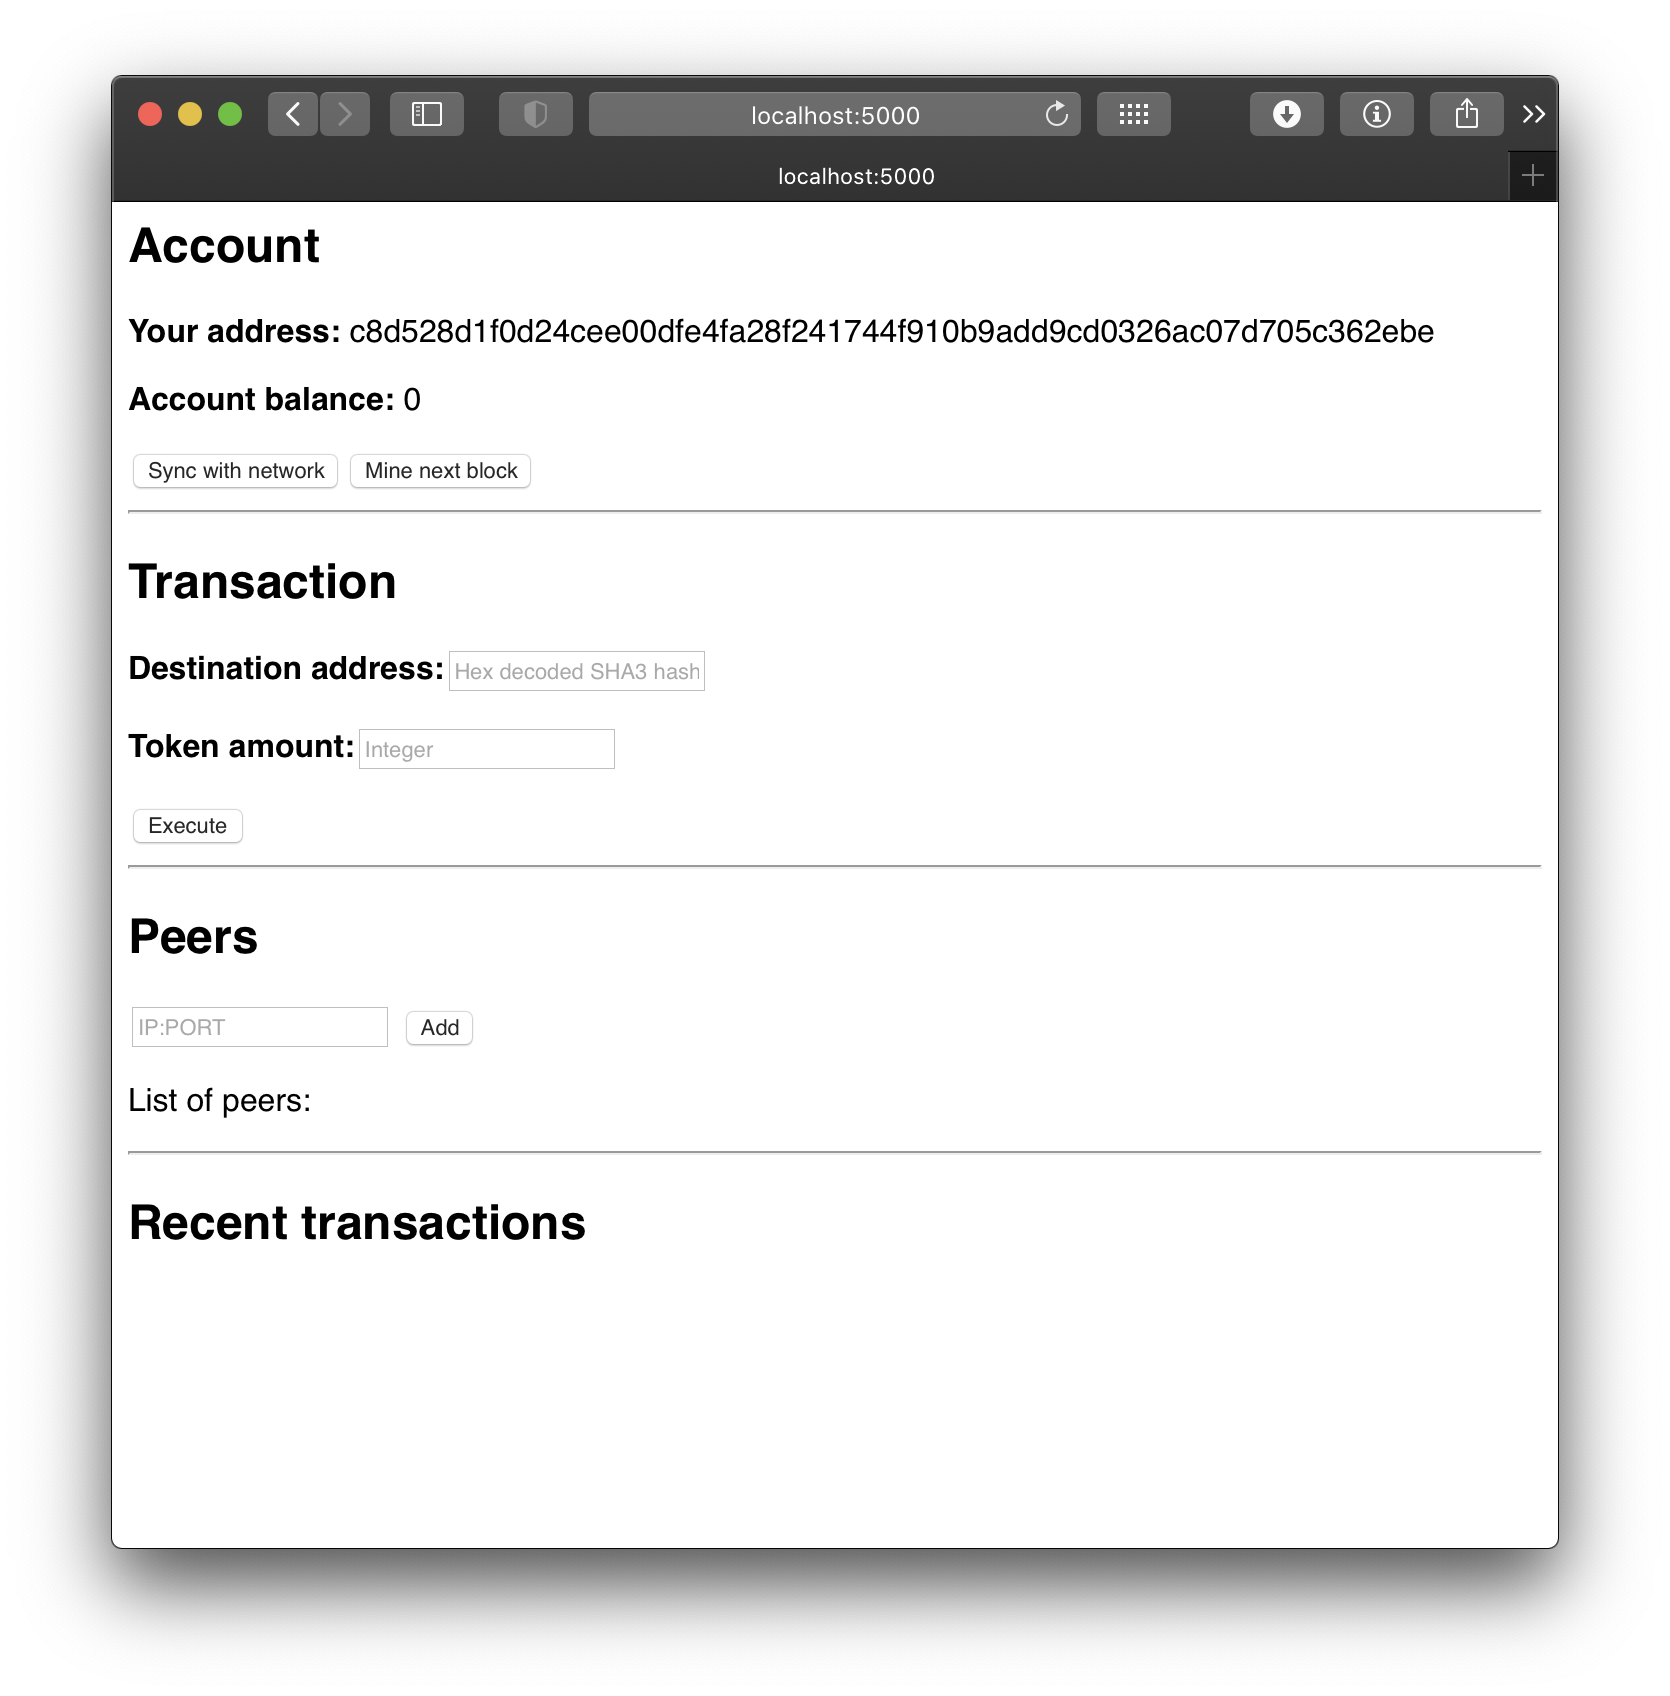
\includegraphics[width=\textwidth]{sucelje}
%     \caption{Izgled korisničkog sučelja}
%     \label{fig:sucelje}
% \end{figure}

% \begin{figure}[htp]
%     \centering
%     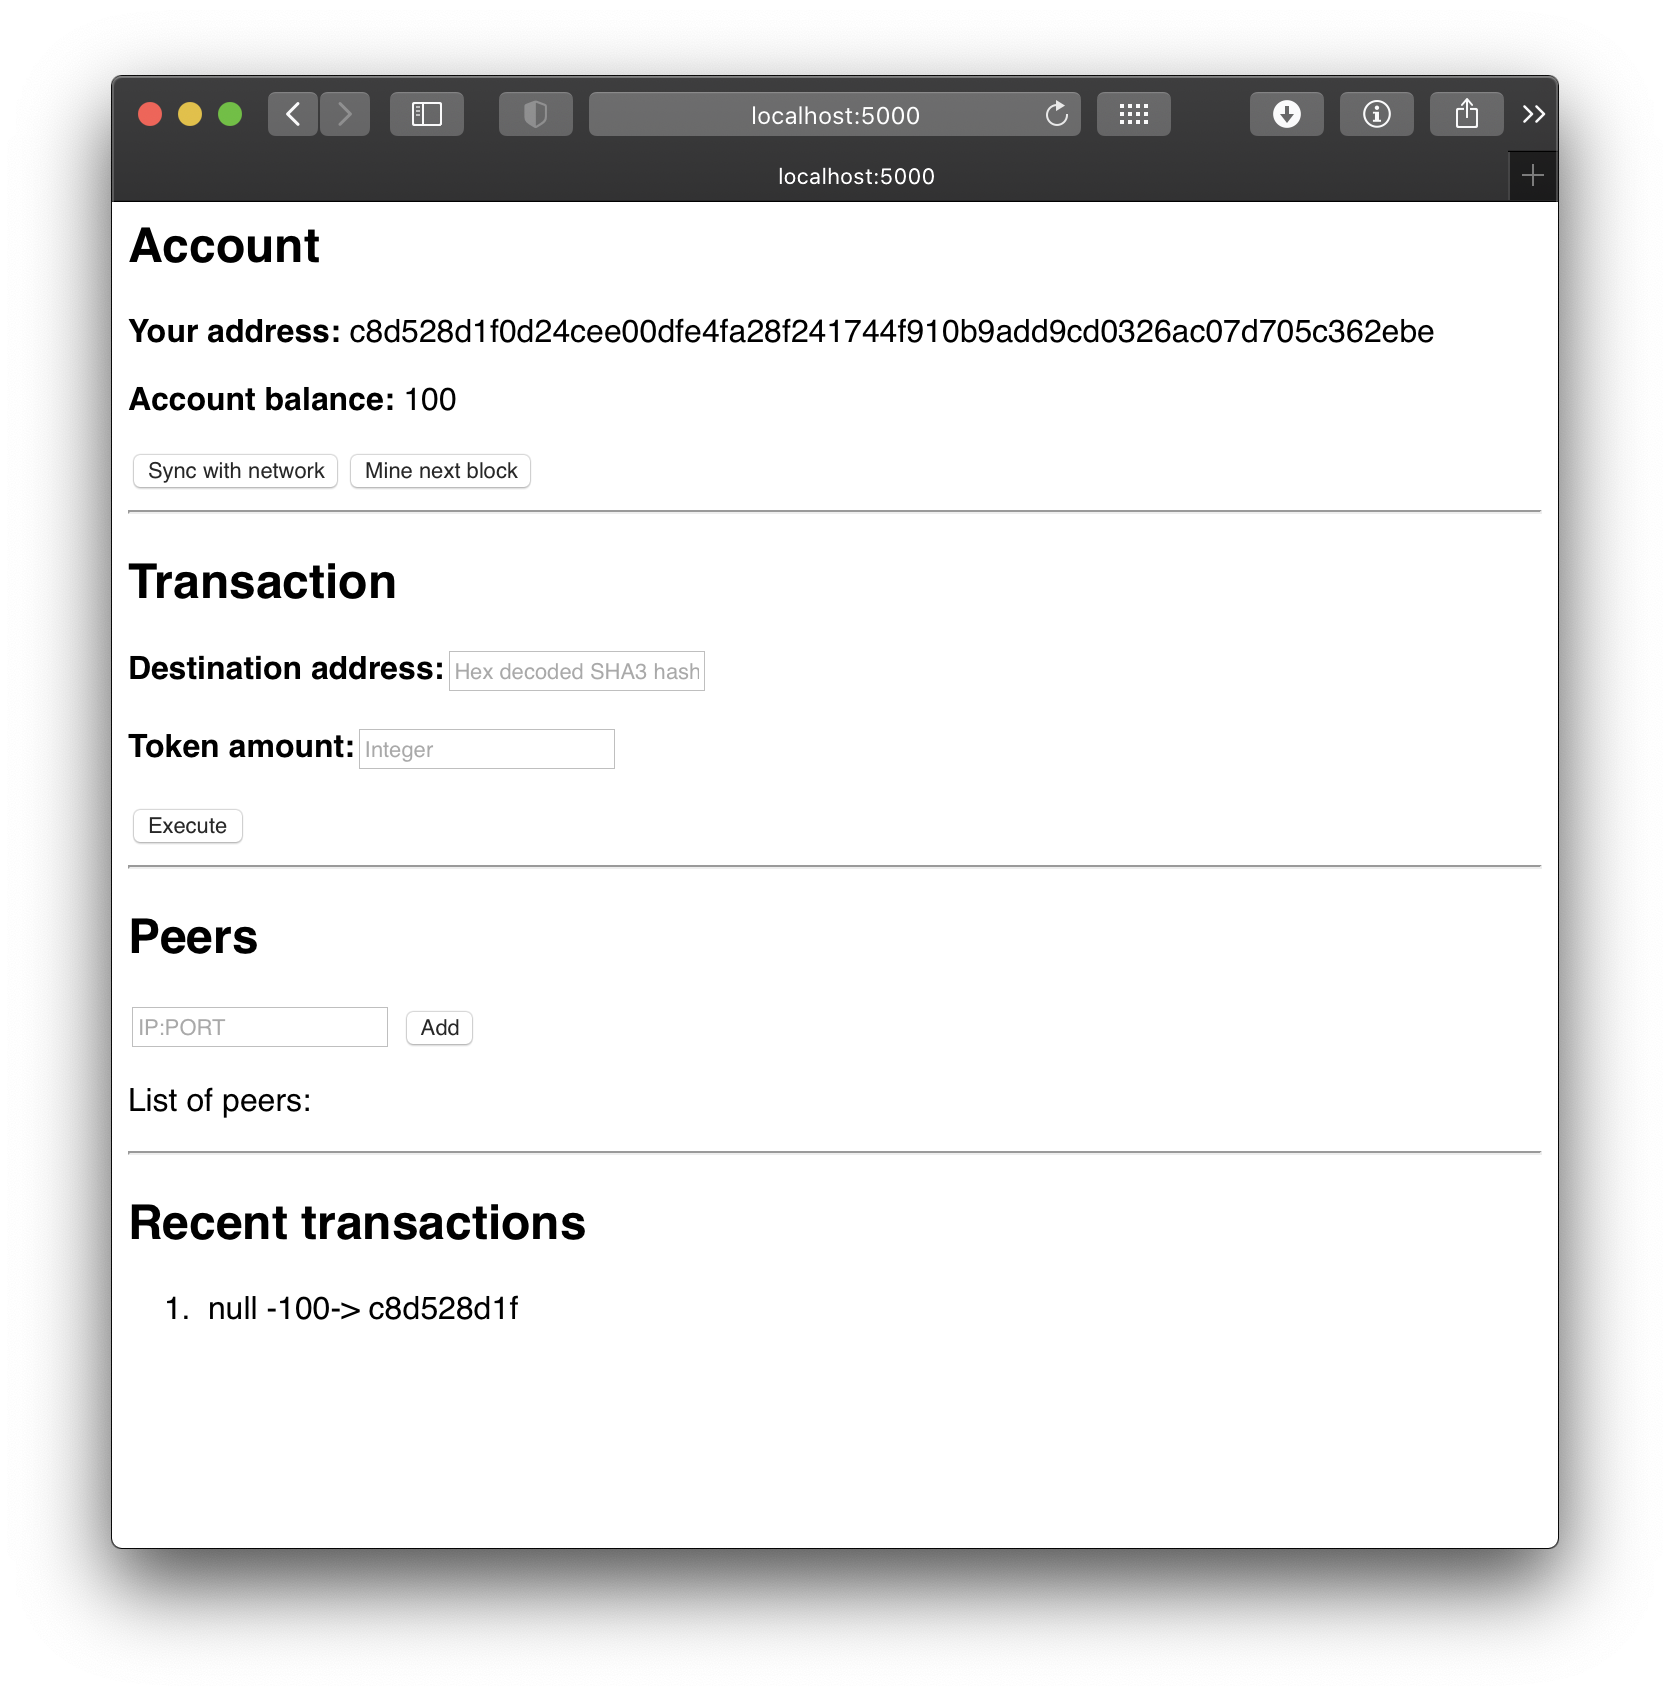
\includegraphics[width=\textwidth]{rudarenje}
%     \caption{Rudarenje stranice}
%     \label{fig:rudarenje}
% \end{figure}

% \begin{figure}[htp]
%     \centering
%     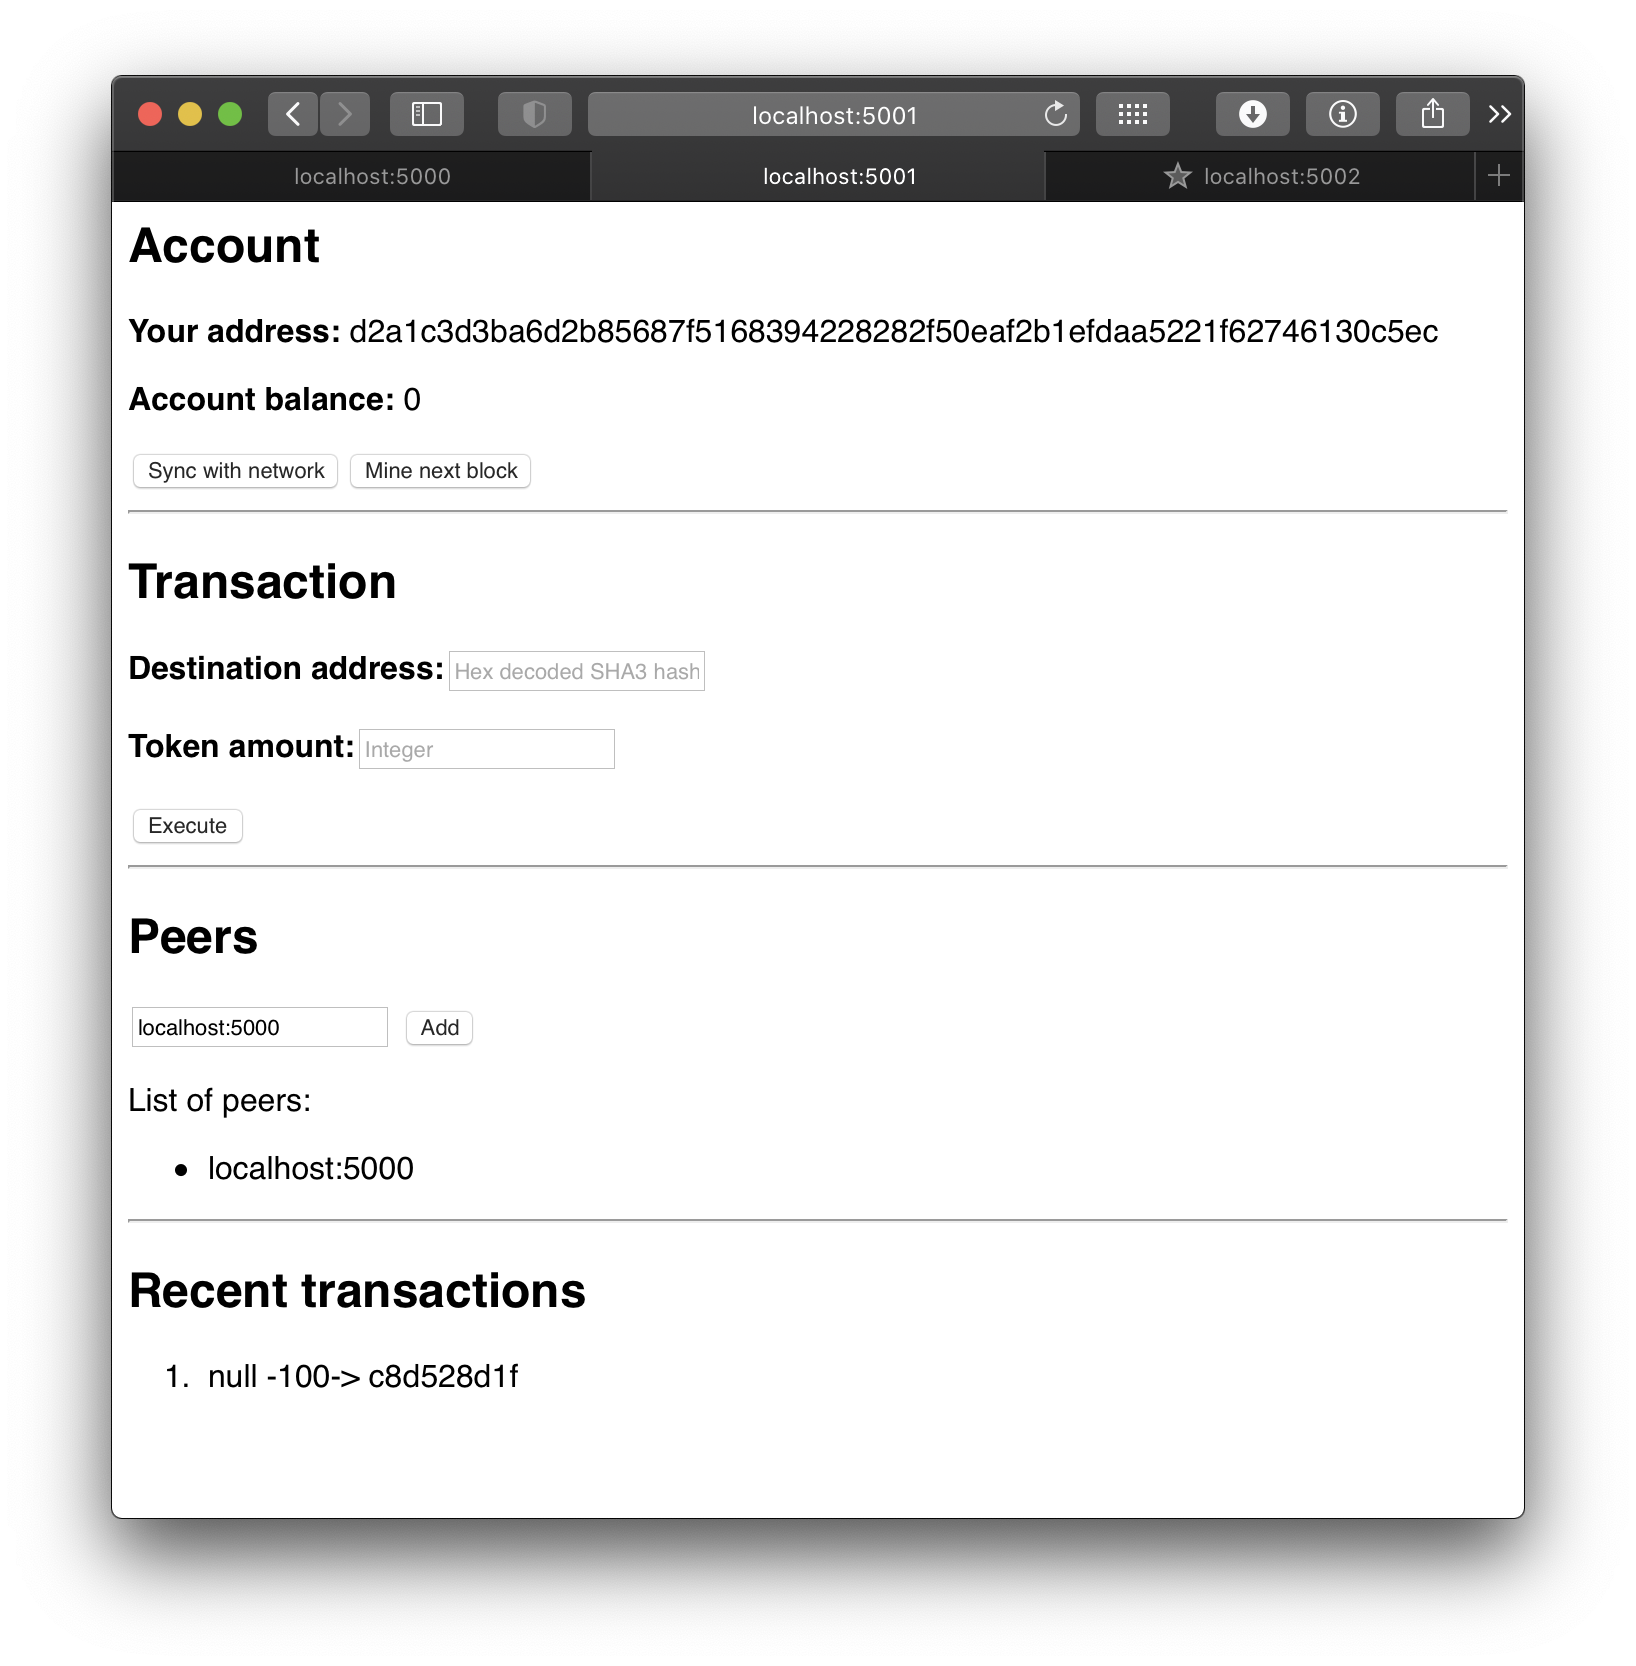
\includegraphics[width=\textwidth]{dodavanje_ip_adrese_susjeda.png}
%     \caption{Dodavanje susjednih čvorova}
%     \label{fig:dodaj_ip}
% \end{figure}

% \begin{figure}[htp]
%     \centering
%     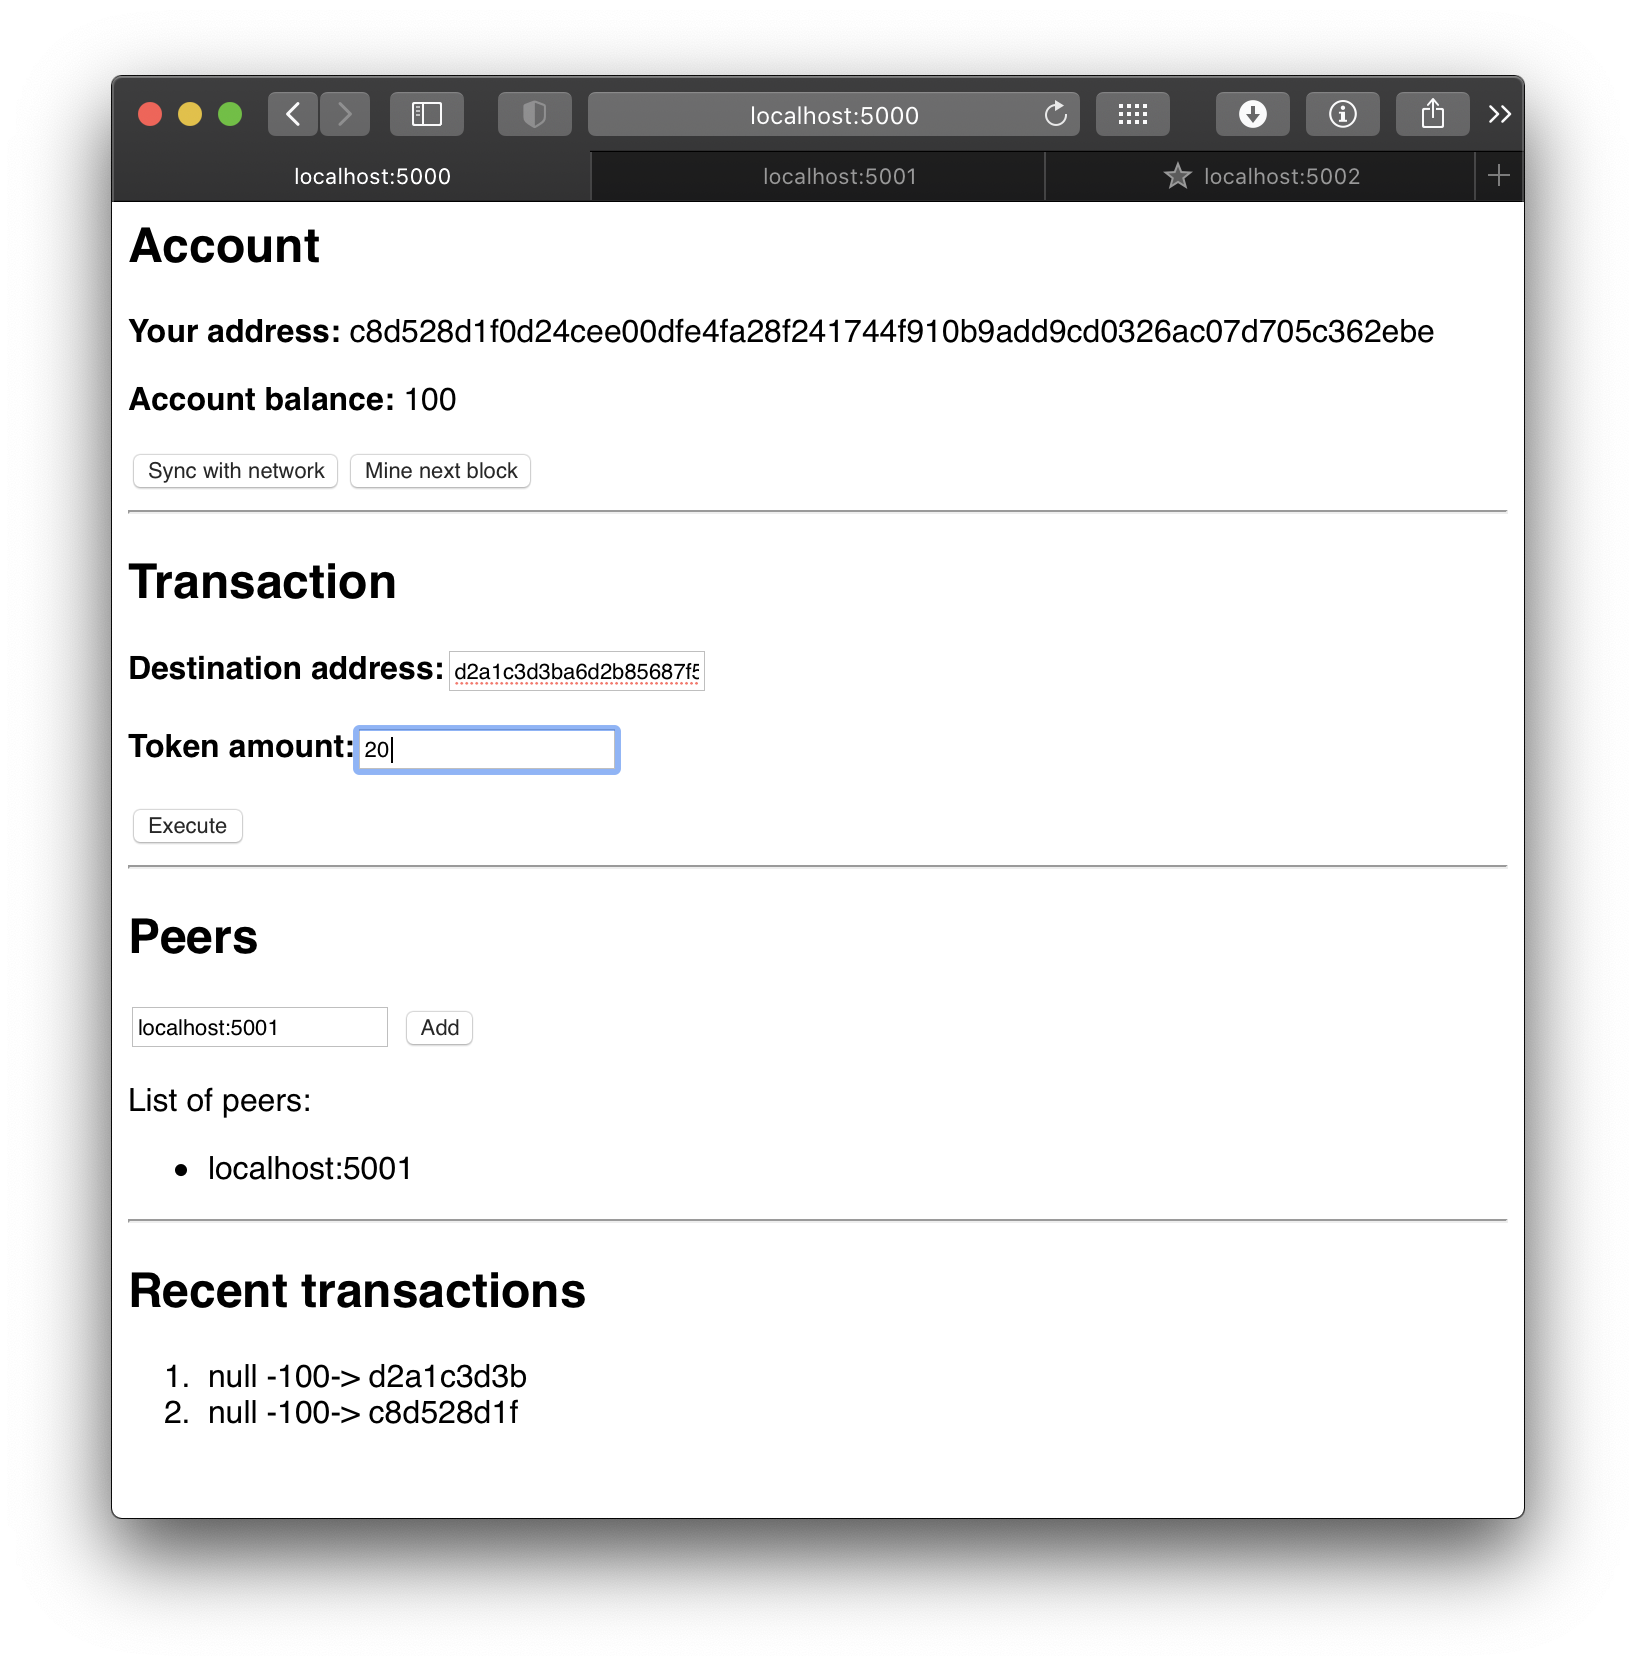
\includegraphics[width=\textwidth]{transakcija.png}
%     \caption{Slanje novca}
%     \label{fig:transakcija}
% \end{figure}

% \begin{figure}[htp]
%     \centering
%     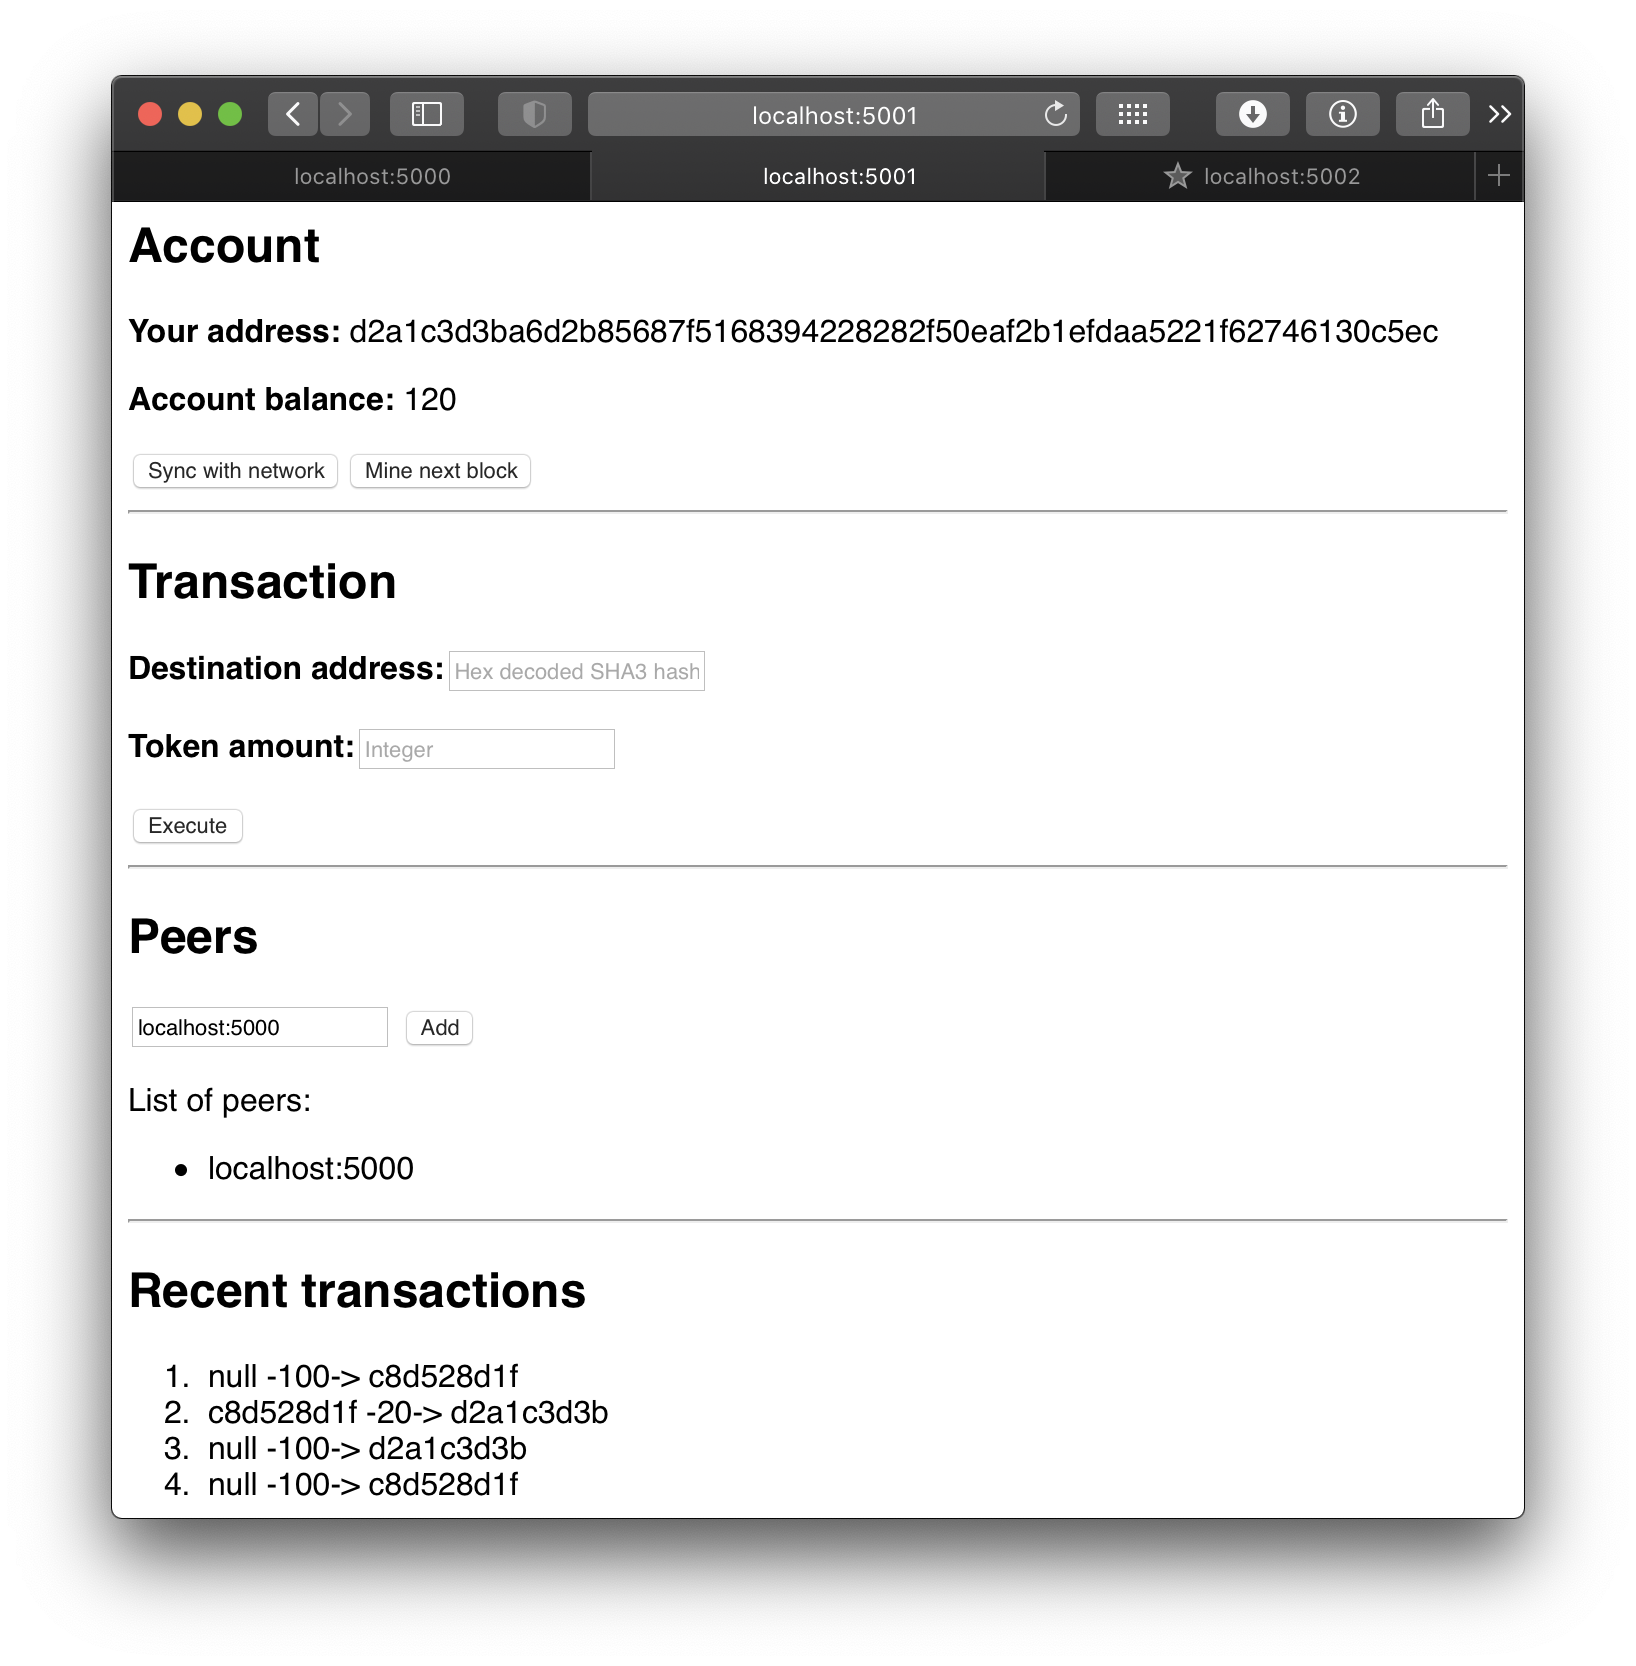
\includegraphics[width=\textwidth]{sinkronizacija.png}
%     \caption{Sinkronizacija sa početnim čvorom kako bismo vidjeli primljeni iznos}
%     \label{fig:sinkronizacija}
% \end{figure}

% \begin{figure}[htp]
%     \centering
%     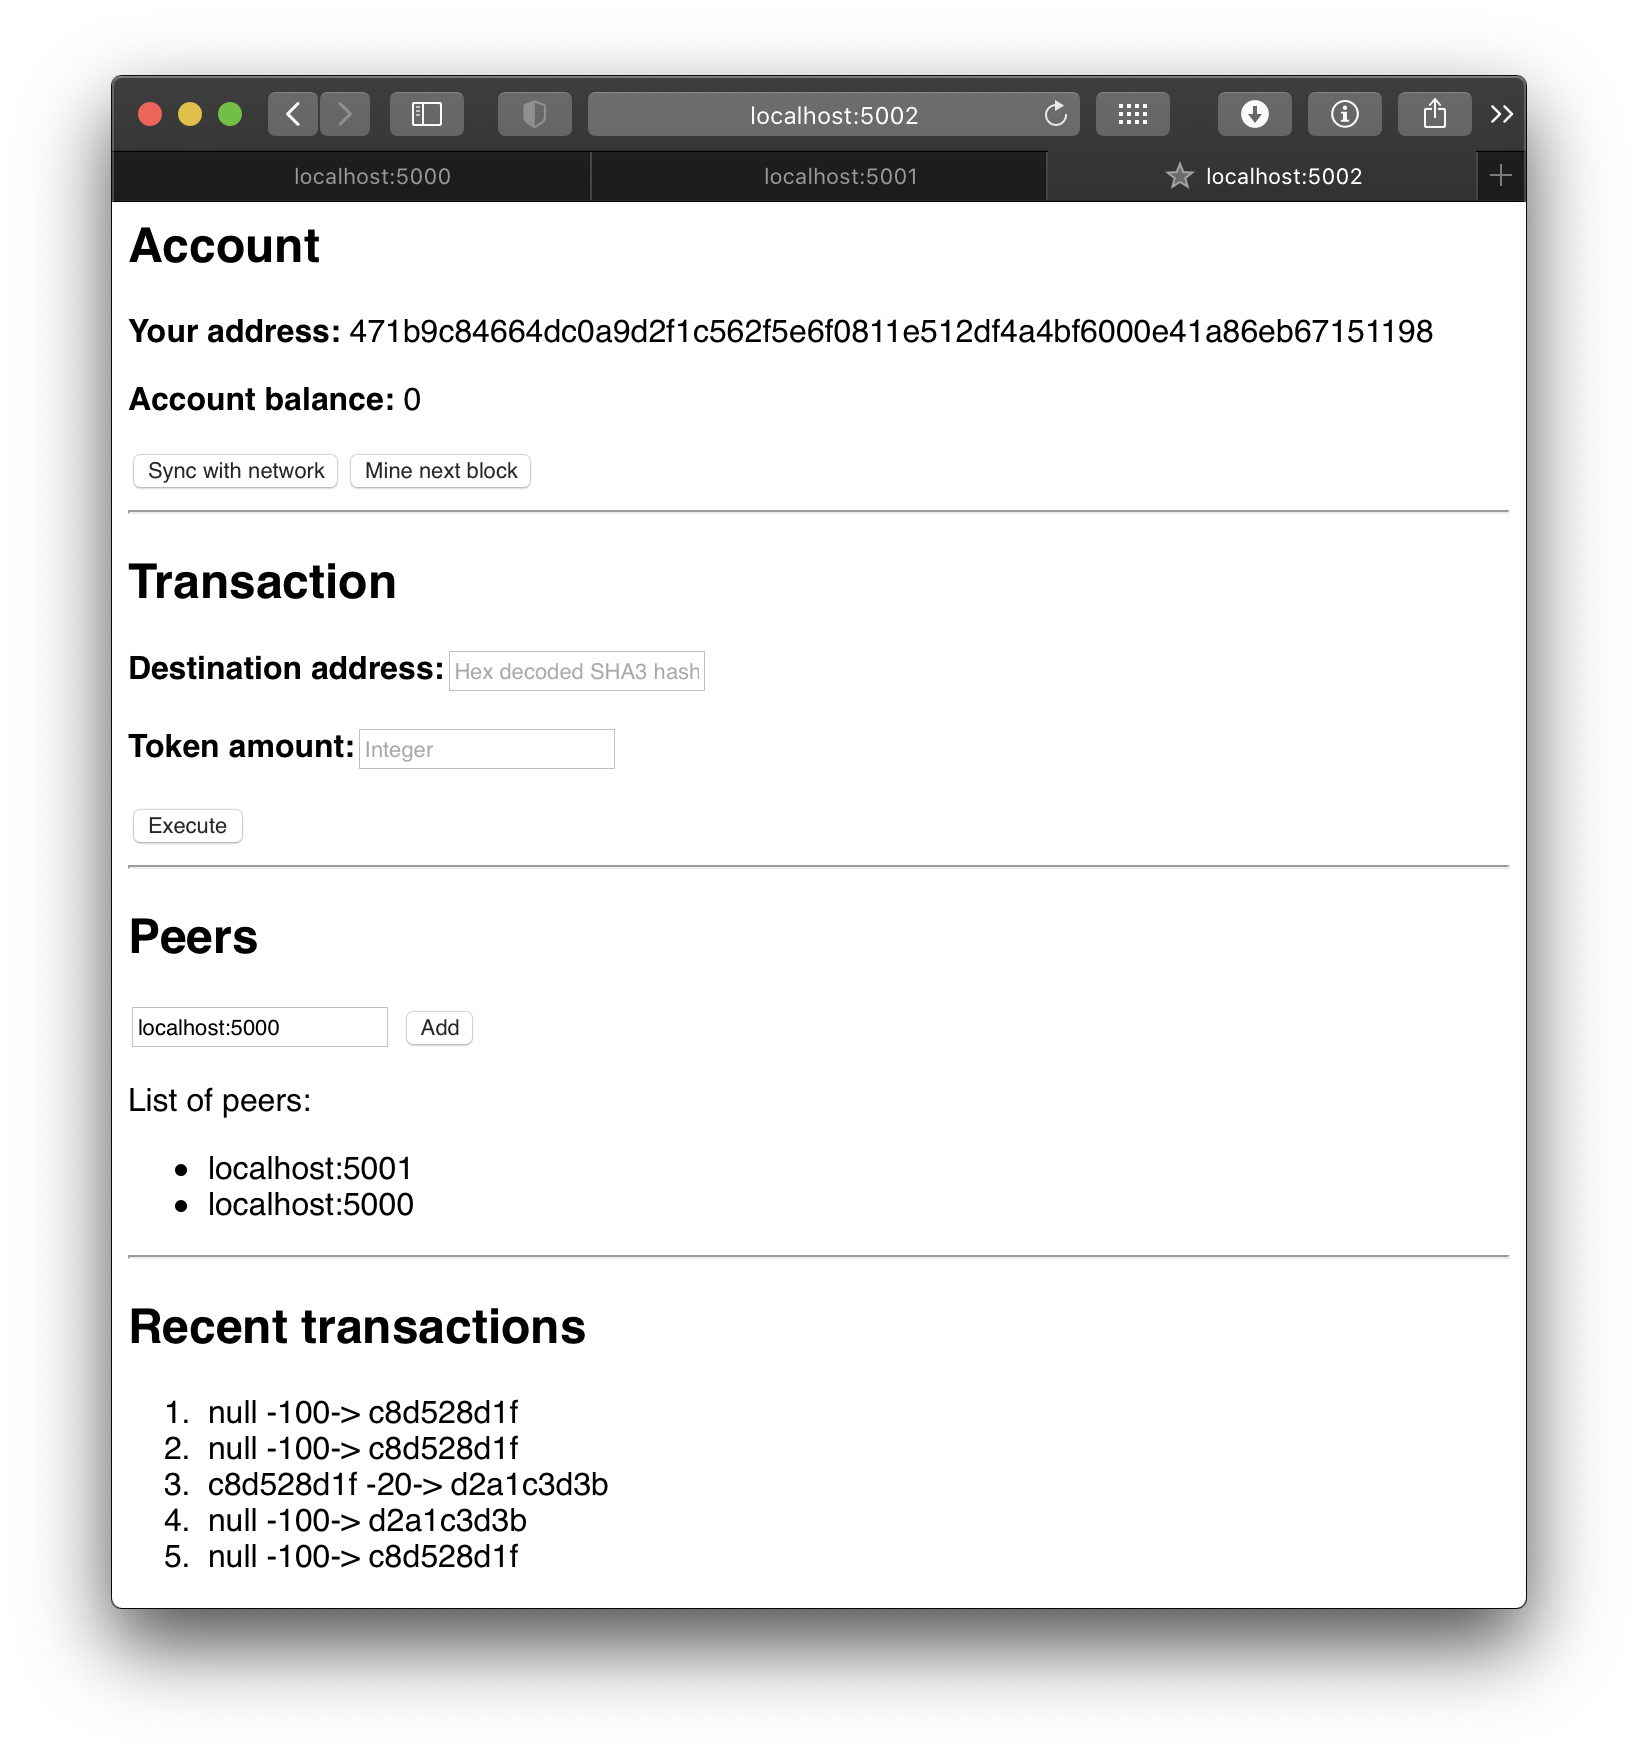
\includegraphics[width=\textwidth]{autoritativni_najdulji_lanac.png}
%     \caption{Odabir autoritativnog lanca na trećem čvoru}
%     \label{fig:autoritativni}
% \end{figure}

% =========================
\chapter{Zaključak}
Zaključak.

\bibliographystyle{fer}
\bibliography{literatura}


\begin{sazetak}
	Obrađujemo temu lanca stranica i simuliramo rad kriptovalute te postizanje suglasja između više čvorova u mreži. Objašnjavaju se pojmovi središnjeg autoriteta, suglasje u sustavima bez povjerenja, digitalno potpisivanje i validacija transakcija u sustavima lanca stranica.

\kljucnerijeci{Ključne riječi, odvojene zarezima.}
\end{sazetak}

% TODO: Navedite naslov na engleskom jeziku.
\engtitle{Blockchain and distributed consensus in electronic money systems}
\begin{abstract}
	
\keywords{Lanac stranica, distribuirano suglasje, digitalni potpis, elektronički novac}
\end{abstract}

\end{document}